\documentclass{standalone}
\usepackage{tikz}
\usetikzlibrary{patterns, positioning}

\begin{document}
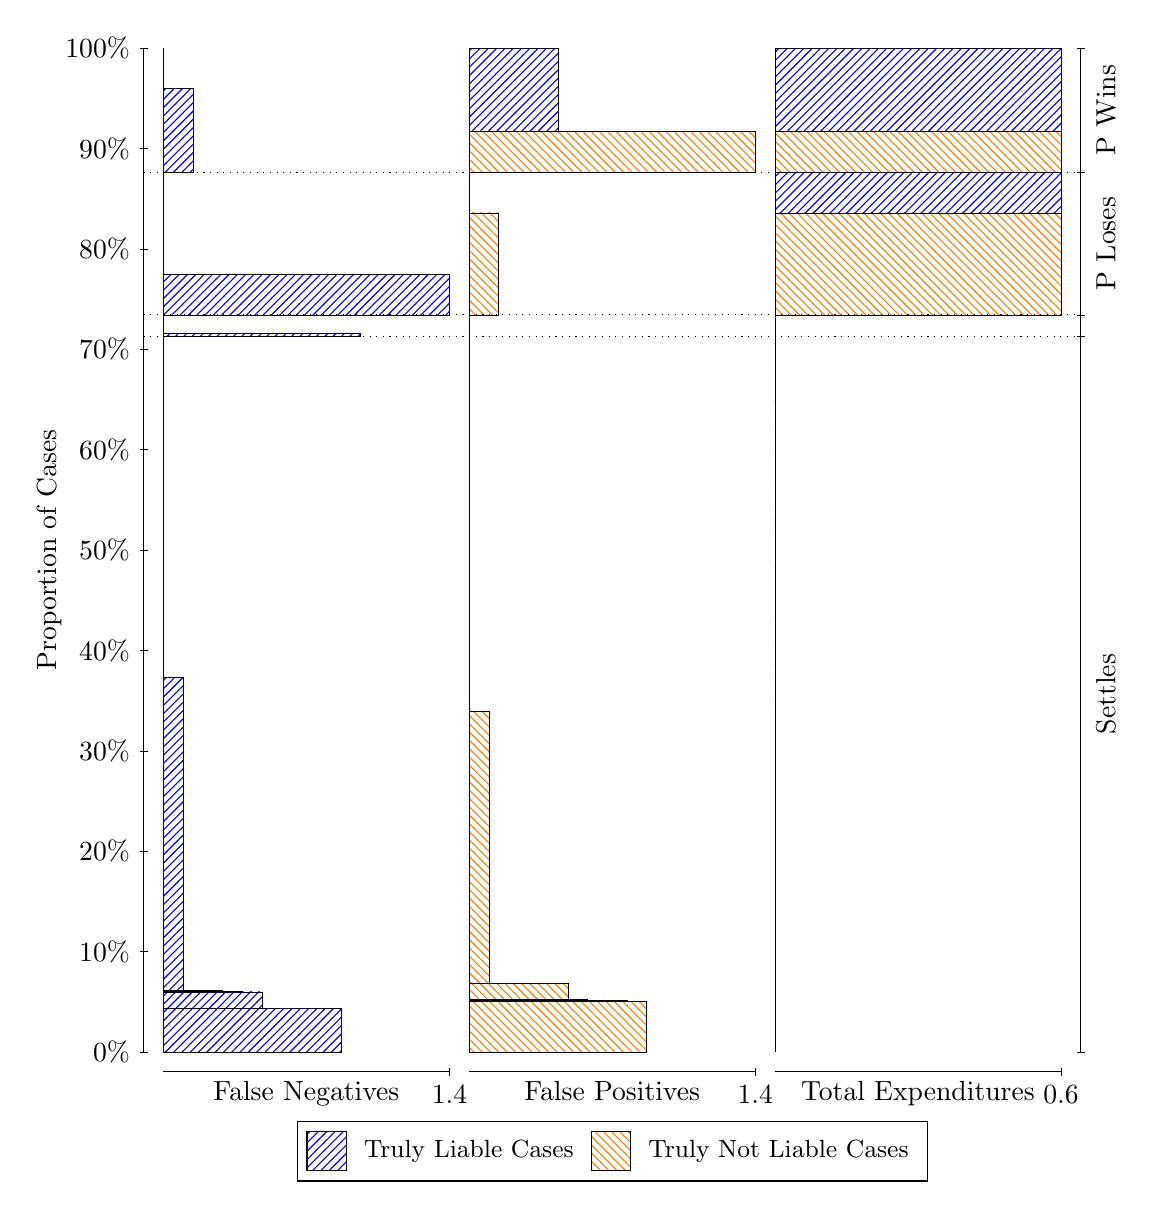
\begin{tikzpicture}
\draw[black, very thin] (1.5,1.75) -- (1.5,14.5);
\node[rotate=90, anchor=center] at (0.3, 8.125) {Proportion of Cases};
\draw[black, very thin] (1.45,1.75) -- (1.55,1.75);
\node[anchor=east] at (1.45, 1.75) {0\%};
\draw[black, very thin] (1.45,3.025) -- (1.55,3.025);
\node[anchor=east] at (1.45, 3.025) {10\%};
\draw[black, very thin] (1.45,4.3) -- (1.55,4.3);
\node[anchor=east] at (1.45, 4.3) {20\%};
\draw[black, very thin] (1.45,5.575) -- (1.55,5.575);
\node[anchor=east] at (1.45, 5.575) {30\%};
\draw[black, very thin] (1.45,6.85) -- (1.55,6.85);
\node[anchor=east] at (1.45, 6.85) {40\%};
\draw[black, very thin] (1.45,8.125) -- (1.55,8.125);
\node[anchor=east] at (1.45, 8.125) {50\%};
\draw[black, very thin] (1.45,9.4) -- (1.55,9.4);
\node[anchor=east] at (1.45, 9.4) {60\%};
\draw[black, very thin] (1.45,10.675) -- (1.55,10.675);
\node[anchor=east] at (1.45, 10.675) {70\%};
\draw[black, very thin] (1.45,11.95) -- (1.55,11.95);
\node[anchor=east] at (1.45, 11.95) {80\%};
\draw[black, very thin] (1.45,13.225) -- (1.55,13.225);
\node[anchor=east] at (1.45, 13.225) {90\%};
\draw[black, very thin] (1.45,14.5) -- (1.55,14.5);
\node[anchor=east] at (1.45, 14.5) {100\%};

\draw[black, very thin] (13.4,1.75) -- (13.4,14.5);
\draw[black, very thin] (13.35,1.75) -- (13.45,1.75);
\node[anchor=west] at (13.35, 1.75) {};
\draw[black, very thin] (13.35,10.84) -- (13.45,10.84);
\node[anchor=west] at (13.35, 10.84) {};
\draw[black, very thin] (13.35,11.112) -- (13.45,11.112);
\node[anchor=west] at (13.35, 11.112) {};
\draw[black, very thin] (13.35,12.923) -- (13.45,12.923);
\node[anchor=west] at (13.35, 12.923) {};
\draw[black, very thin] (13.35,14.5) -- (13.45,14.5);
\node[anchor=west] at (13.35, 14.5) {};

\draw[black, very thin, pattern color=blue, pattern=north east lines] (1.75,1.75) rectangle (4.0052,2.3049);
\draw[black, very thin, pattern color=blue, pattern=north east lines] (1.75,2.3049) rectangle (3.0029,2.5144);
\draw[black, very thin, pattern color=blue, pattern=north east lines] (1.75,2.5144) rectangle (2.7523,2.5217);
\draw[black, very thin, pattern color=blue, pattern=north east lines] (1.75,2.5217) rectangle (2.5017,2.5291);
\draw[black, very thin, pattern color=blue, pattern=north east lines] (1.75,2.5291) rectangle (2.2511,2.5366);
\draw[black, very thin, pattern color=blue, pattern=north east lines] (1.75,2.5366) rectangle (2.0006,6.5106);
\draw[black, very thin, pattern color=orange, pattern=north west lines] (1.75,6.5106) rectangle (1.75,10.84);
\draw[black, very thin, pattern color=blue, pattern=north east lines] (1.75,10.84) rectangle (4.2557,10.875);
\draw[black, very thin, pattern color=orange, pattern=north west lines] (1.75,10.875) rectangle (1.75,11.112);
\draw[black, very thin, pattern color=blue, pattern=north east lines] (1.75,11.112) rectangle (5.3833,11.628);
\draw[black, very thin, pattern color=orange, pattern=north west lines] (1.75,11.628) rectangle (1.75,12.923);
\draw[black, very thin, pattern color=blue, pattern=north east lines] (1.75,12.923) rectangle (2.1259,13.985);
\draw[black, very thin, pattern color=orange, pattern=north west lines] (1.75,13.985) rectangle (1.75,14.5);
\draw[black, very thin, pattern color=orange, pattern=north west lines] (5.6333,1.75) rectangle (7.8885,2.3929);
\draw[black, very thin, pattern color=orange, pattern=north west lines] (5.6333,2.3929) rectangle (7.6379,2.4005);
\draw[black, very thin, pattern color=orange, pattern=north west lines] (5.6333,2.4005) rectangle (7.3874,2.408);
\draw[black, very thin, pattern color=orange, pattern=north west lines] (5.6333,2.408) rectangle (7.1368,2.4154);
\draw[black, very thin, pattern color=orange, pattern=north west lines] (5.6333,2.4154) rectangle (6.8862,2.6244);
\draw[black, very thin, pattern color=orange, pattern=north west lines] (5.6333,2.6244) rectangle (5.8839,6.079);
\draw[black, very thin, pattern color=blue, pattern=north east lines] (5.6333,6.079) rectangle (5.6333,10.84);
\draw[black, very thin, pattern color=orange, pattern=north west lines] (5.6333,10.84) rectangle (5.6333,11.076);
\draw[black, very thin, pattern color=blue, pattern=north east lines] (5.6333,11.076) rectangle (5.6333,11.112);
\draw[black, very thin, pattern color=orange, pattern=north west lines] (5.6333,11.112) rectangle (6.0092,12.407);
\draw[black, very thin, pattern color=blue, pattern=north east lines] (5.6333,12.407) rectangle (5.6333,12.923);
\draw[black, very thin, pattern color=orange, pattern=north west lines] (5.6333,12.923) rectangle (9.2667,13.438);
\draw[black, very thin, pattern color=blue, pattern=north east lines] (5.6333,13.438) rectangle (6.7609,14.5);
\draw[black, very thin, pattern color=orange, pattern=north west lines] (9.5167,1.75) rectangle (9.5167,6.079);
\draw[black, very thin, pattern color=blue, pattern=north east lines] (9.5167,6.079) rectangle (9.5167,10.84);
\draw[black, very thin, pattern color=orange, pattern=north west lines] (9.5167,10.84) rectangle (9.5167,11.076);
\draw[black, very thin, pattern color=blue, pattern=north east lines] (9.5167,11.076) rectangle (9.5167,11.112);
\draw[black, very thin, pattern color=orange, pattern=north west lines] (9.5167,11.112) rectangle (13.15,12.407);
\draw[black, very thin, pattern color=blue, pattern=north east lines] (9.5167,12.407) rectangle (13.15,12.923);
\draw[black, very thin, pattern color=orange, pattern=north west lines] (9.5167,12.923) rectangle (13.15,13.438);
\draw[black, very thin, pattern color=blue, pattern=north east lines] (9.5167,13.438) rectangle (13.15,14.5);
\draw[black, dotted] (1.5,10.84) -- (13.4,10.84);
\draw[black, dotted] (1.5,11.112) -- (13.4,11.112);
\draw[black, dotted] (1.5,12.923) -- (13.4,12.923);
\draw[black, very thin] (1.75,1.5) -- (5.3833,1.5);
\node[anchor=north] at (3.5667, 1.5) {False Negatives};
\draw[black, very thin] (5.3833,1.45) -- (5.3833,1.55);
\node[anchor=north] at (5.3833, 1.45) {1.4};

\draw[black, very thin] (5.6333,1.5) -- (9.2667,1.5);
\node[anchor=north] at (7.45, 1.5) {False Positives};
\draw[black, very thin] (9.2667,1.45) -- (9.2667,1.55);
\node[anchor=north] at (9.2667, 1.45) {1.4};

\draw[black, very thin] (9.5167,1.5) -- (13.15,1.5);
\node[anchor=north] at (11.333, 1.5) {Total Expenditures};
\draw[black, very thin] (13.15,1.45) -- (13.15,1.55);
\node[anchor=north] at (13.15, 1.45) {0.6};

\node[black, centered, rotate=90] at (13.72, 6.2948) {Settles};

\node[black, centered, rotate=90] at (13.72, 12.017) {P Loses};
\node[black, centered, rotate=90] at (13.72, 13.711) {P Wins};

\draw (7.449999999999999,1.5) node[draw=none] (baseCoordinate) {};
\begin{scope}[align=center]
        \matrix[scale=0.5, draw=black, below=0.5cm of baseCoordinate, nodes={draw}, column sep=0.1cm]{
            \node[rectangle, draw, minimum width=0.5cm, minimum height=0.5cm, pattern=north east lines, pattern color=blue] {}; &
            \node[draw=none, font=\small] (B) {Truly Liable Cases}; &
            \node[rectangle, draw, minimum width=0.5cm, minimum height=0.5cm, pattern=north west lines, pattern color=orange] {}; &
            \node[draw=none, font=\small] (B) {Truly Not Liable Cases}; \\
            };
\end{scope}

\end{tikzpicture}
\end{document}